\subsubsection{Definicija zahtev aplikacije}

Big data aplikacije potrebutjo za svoje delovanje
tudi zunanje storitve, katere želimo postavljati skupaj z
aplikacijo.
V tem odseku bomo analizirali zahteve aplikacije in
iz njih zgradili arhitekturo.

Za začetek potrebujemo poslovno definicijo aplikacije.
Magistrska naloga predpostavlja, da je arhitektura
predstavljena v modelu ArchiMate, ampak od njega ni odvisna.
Arhitekturo bomo razvili za generično aplikacijo,
nato pa jo v poglavju~\ref{sec:uporaba-metodologije} uporabili
na primeru big data aplikacije.
Začnemo z definicijo big data aplikacije.
Aplikacija je sestavljena iz več procesov, kjer ima lahko
vsak proces več zahtev po zunanjih storitvah.
Generična predstavitev je predstavljena v sliki~\ref{fig:generic-arch-application}.

\begin{figure}[H]
    \centering
    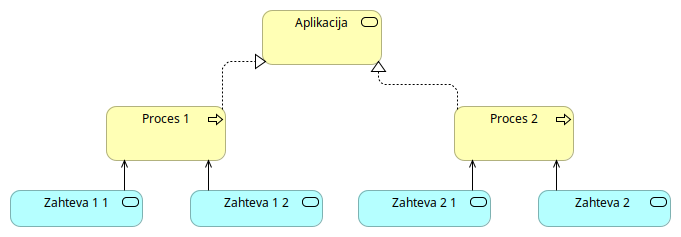
\includegraphics[width=0.9\textwidth]{img/gradnja/generic-arch-application.png}
    \caption{Predstavitev generične arhitekture v modelu Archimate.}
    \label{fig:generic-arch-application}
\end{figure}

Procesi in zahteve imajo lahko posebne lastnosti,
ki omejujejo izbor zunanjih storitev.
Lastnosti lahko definiramo sami, nekateri primeri so predstavljeni v tabeli 1 v članku~\cite{iterative_methodology},
kjer lastnosti storitev definirajo iz lastnosti big data,
ki smo jih predstavili v odseku~\ref{sec:big-data}.
Primeri lastnosti so na primer:
\begin{itemize}
    \item Volumen podatkov
    \item Hitrost podatkovnih tokov
    \item Raznolikost podatkov
    \item Zaupanje v podatke
    \item Strukturiranost podatkov
\end{itemize}

Lastnosti so lahko prisotne ali ne, na primer ali neka baza podpira nestrukturirane podatke ali ne,
ter prisotne na spektru, na primer kako hitro deluje.
Za arhitekturo v tem poglavju želimo, da bo aplikacija visoko dostopna.
V naši generični predstavitvi ta primer predstavimo s procesom 1 in pomeni,
da mora biti proces 1 in njegove zahteve visoko dostopni.
Dodana omejitev je predstavljena v sliki~\ref{fig:generic-arch-application-labels}.

\begin{figure}[H]
    \centering
    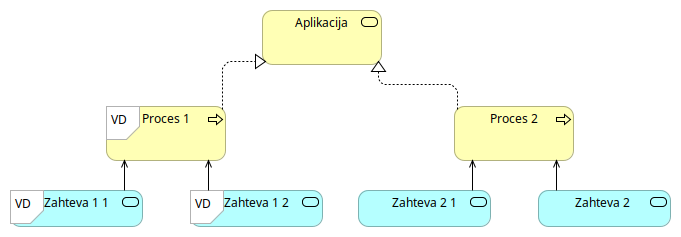
\includegraphics[width=0.9\textwidth]{img/gradnja/generic-arch-application-labels.png}
    \caption{Arhitektura z lastnostjo zahtev in procesov.}
    \label{fig:generic-arch-application-labels}
\end{figure}

V naslednjem koraku izpolnimo zahteve.
V prejšnjem koraku smo zahteve označili z lastnostmi in sedaj je naša
izbira tehnologij omejena na tiste, ki ustrezajo tem lastnostim.
Med ustreznimi tehnologijami se odločimo za tisto,
ki najbolj ustreza še drugim zahtevam, ki ne izvirajo nujno samo iz
same aplikacije, na primer da izberemo tehnologijo, ki jo naše podjetje
že pozna.
Po izbiri dodamo zunanje storitve v arhitekturo.
Ena storitev lahko zadostuje več zahtevam,
če zadostuje tudi njihovim lastnostim.
Arhitektura po dodatku storitev je predstavljena v sliki~\ref{fig:generic-services}.

\begin{figure}[H]
    \centering
    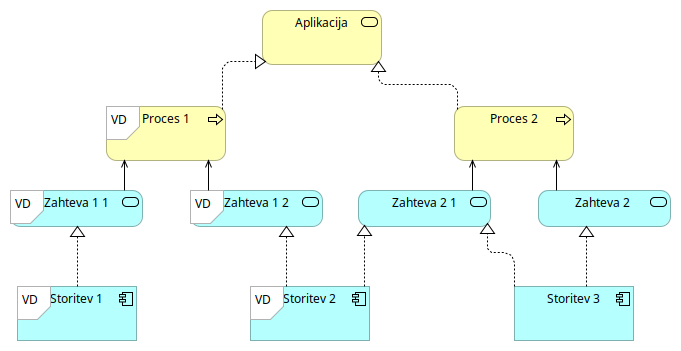
\includegraphics[width=0.9\textwidth]{img/gradnja/generic-services.png}
    \caption{Arhitektura s storitvami.}
    \label{fig:generic-services}
\end{figure}

V naslednjem odseku predstavimo primere tehnologij in njihove lastnosti.
Predstavili bomo par tehnologij iz vsake skupine in predstavili skupine na splošno.
